\chapter{Исследовательский раздел}

Программное обеспечение было реализовано на дистрибутиве Ubuntu 20.04 \cite{ubuntu}, ядро версии 5.15.60 \cite{kernel}.

\section{Примеры работы разработанного ПО}

Записи о состоянии физических страниц, выделенных процессу, можно прочитать в системном журнале. Для этого необходимо выполнить команду~(листинг \ref{lst:dmesg.txt}):

\includelisting
    {dmesg.txt}
    {Команда получения записей в системном журнале о состоянии физических страниц, выделенных процессу}
    
На рисунке \ref{img:example1} представлен пример результата работы загружаемого модуля ядра --- мониторинг состояния физических страниц процесса с pid, равным 17010. Для наглядности представлена часть записей.

\begin{figure}[H]
	\begin{center}
		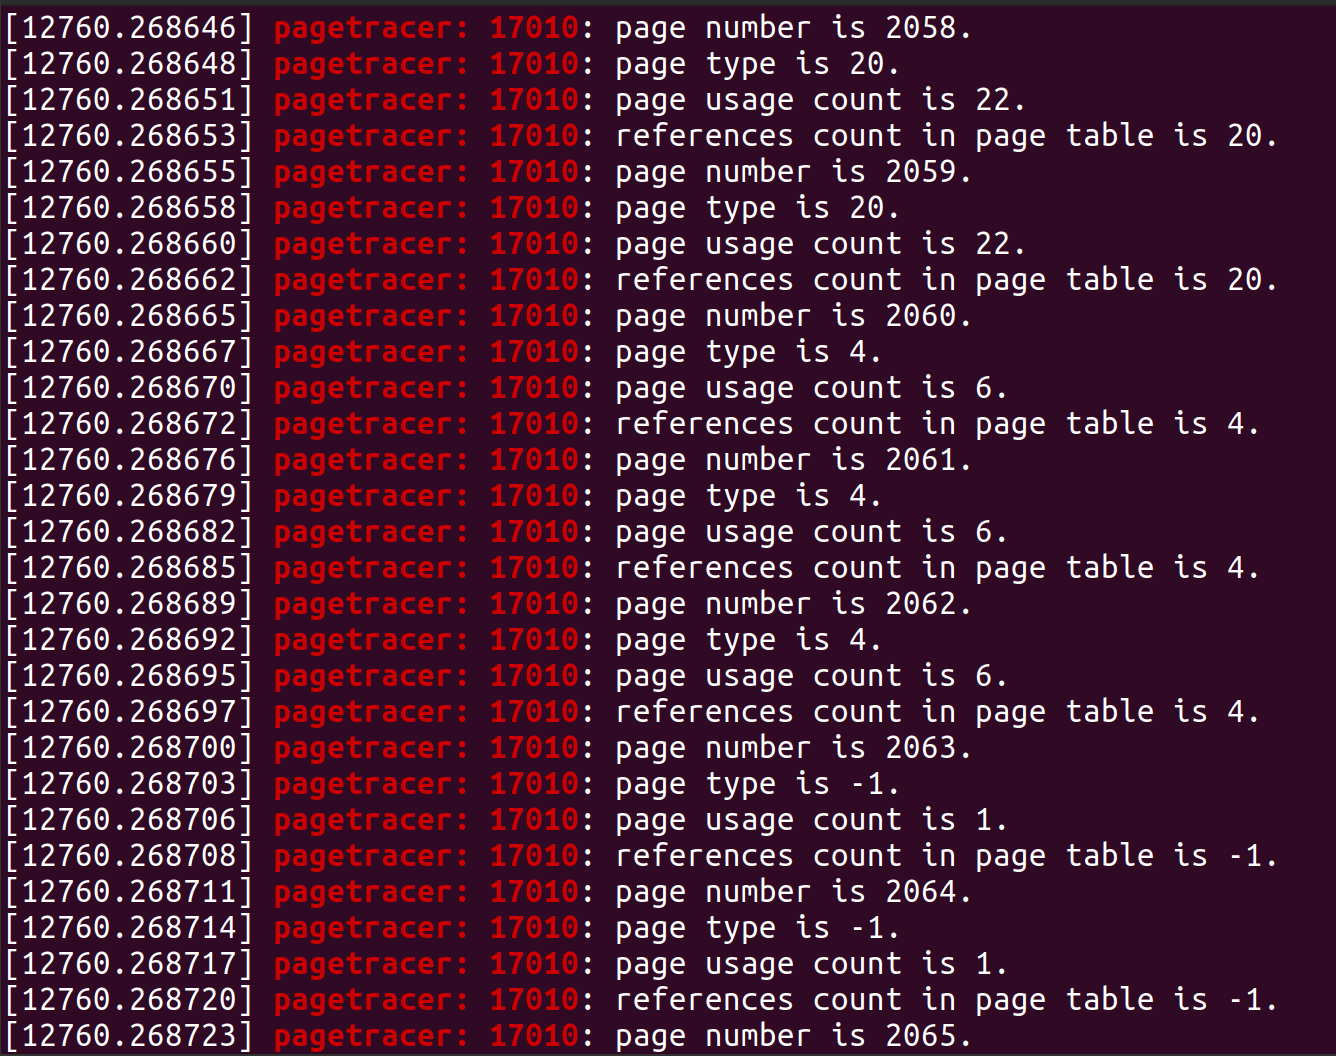
\includegraphics[scale=0.42]{inc/img/example1.png}
	\end{center}
	\captionsetup{justification=centering}
	\caption{Мониторинг состояния физических страниц процесса с pid, равным 17010}
	\label{img:example1}
\end{figure}

На рисунке \ref{img:example2} показана ситуация, когда идентификатор процесса не был задан при загрузке модуля.
    
\begin{figure}[H]
	\begin{center}
		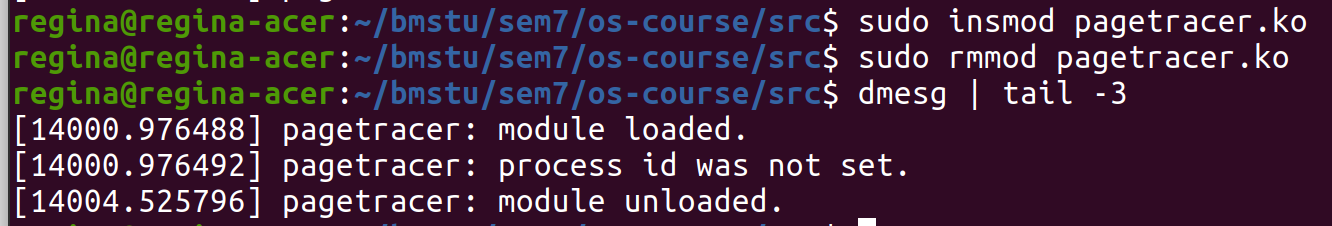
\includegraphics[scale=0.45]{inc/img/example2.png}
	\end{center}
	\captionsetup{justification=centering}
	\caption{Идентификатор процесса не задан при загрузке модуля}
	\label{img:example2}
\end{figure}
